%%%%%%%%%%%%%%%%%%%%%%%%%%%%%%%%%%%%%%%%%%%%%%%%%%%%%%%%%%%%%%%%%%%%%%%%%%%%

\documentclass[10pt]{article}

\usepackage{amssymb, graphicx, paralist}
\usepackage[letterpaper,text={7in,9.75in},centering]{geometry}

%	layout

\pagestyle{empty}
\setlength{\parskip}{1.0ex plus0.2ex minus0.2ex}
\setlength{\parindent}{0.0in}
\renewcommand{\baselinestretch}{1.2}

%	definitions

\newcommand{\C}{\mathbb{C}}
\newcommand{\N}{\mathbb{N}}
\newcommand{\R}{\mathbb{R}}
\newcommand{\Z}{\mathbb{Z}}

\newcommand{\rme}{\mathrm{e}}
\newcommand{\rmd}{\mathrm{d}}
\newcommand{\rmD}{\mathrm{D}}

%%%%%%%%%%%%%%%%%%%%%%%%%%%%%%%%%%%%%%%%%%%%%%%%%%%%%%%%%%%%%%%%%%%%%%%%%%%%

\begin{document}

\begin{center}
    \bf
    APMA 1360, Spring 2025, Assignment \#3\\
    Due on Friday, February~14
\end{center}

\underline{\hspace*{\textwidth}}

%%%%%%%%%%%%%%%%%%%%%%%%%%%%%%%%

\textbf{Purpose:} This problem set focuses on bifurcations and singular perturbations. We will hone our skills for identifying bifurcations that are consistent with the dynamics and with the structure of the differential equation. We will also investigate how small parameters in front of the highest derivatives may affect the dynamics.

\textbf{Rubric:}
\begin{compactitem}
    \item Completeness of arguments and calculations
\end{compactitem}

\underline{\hspace*{\textwidth}}

%%%%%%%%%%%%%%%%%%%%%%%%%%%%%%%%

\textbf{\#3.1 (5 points) Classifying bifurcation diagrams}

Consider the following three potential bifurcation diagrams for a differential equation $\dot{x}=f(x,\mu)$ on the line, where stable and unstable equilibria are drawn as solid and dashed curves, respectively. For each diagram, circle all bifurcation points in the $(\mu,x)$-plane and classify them as saddle-node, transcritical, and pitchfork, or argue why the resulting diagram is impossible.
\begin{center}
    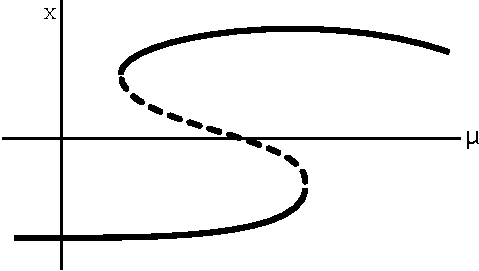
\includegraphics[scale=0.7]{Images/Assignment_Figure_2.pdf}\qquad
    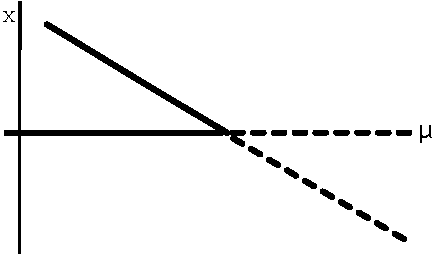
\includegraphics[scale=0.7]{Images/Assignment_Figure_3.pdf}\qquad
    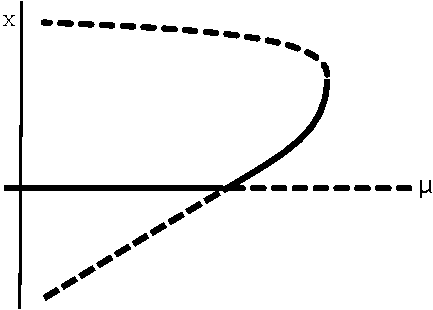
\includegraphics[scale=0.7]{Images/Assignment_Figure_4.pdf}
\end{center}

\underline{\hspace*{\textwidth}}

%%%%%%%%%%%%%%%%%%%%%%%%%%%%%%%%

\textbf{\#3.2 (5 points) Which bifurcations do we expect to encounter?}

Consider the differential equation $\dot{u}=f(u,\mu)$. For each of the different functions listed below, argue whether and why, or why not, you expect to see a saddle-node, pitchfork or transcritical bifurcation to occur at $u=0$ for some value of $\mu$.
\begin{compactenum}[(i)]
    \item $f(u,\mu) = \mu-3u^2$
    \item $f(u,\mu) = \mu u+u\sin u$
    \item $f(u,\mu) = \mu u - u^2\sin u+u^5$
\end{compactenum}
\emph{Note:} you do \textbf{not} need to find bifurcation points or analyse them. It suffices to state which bifurcations you expect to find, which you think cannot occur, and provide arguments that support your statements. In other words, the point of this problem is not to find all bifurcation point explicitly by solving these equations but rather to exclude certain bifurcations, because they should not occur and argue why not.

\underline{\hspace*{\textwidth}}

%%%%%%%%%%%%%%%%%%%%%%%%%%%%%%%%

\textbf{\#3.3 (5 points) Singular perturbations and the implicit function theorem}

This problem will explore the reasons for why we may be able to drop the second-order derivative term in the model of the bead on the rotating hoop. Consider the differential equation
\begin{equation}\label{e1}
    \epsilon \frac{\rmd^2 u}{\rmd t^2} + \frac{\rmd u}{\rmd t} + u = 0.
\end{equation}
\begin{compactenum}[(i)]
    \item Show that $u(t)=u_0\rme^{-t}$ is the general solution of the equation $\dot{u}+u=0$, that is (\ref{e1}) with $\epsilon=0$.
    \item Show that $u(t)=u_1\rme^{\lambda t}$ is a solution of (\ref{e1}) for each value of $u_1$ if, and only if, $\epsilon\lambda^2+\lambda+1=0$.
    \item Use the implicit function theorem to prove that there is a solution of the form $u(t)=u_1 \rme^{\lambda_1(\epsilon)t}$ where $\lambda_1(\epsilon)=-1+O(\epsilon)$ is $C^\infty$.
    \item Show that for each $\varepsilon>0$ there is a second solution of the form $u(t)=u_2\rme^{\lambda_2(\epsilon)t/\epsilon}$ for arbitrary $u_2$ where $\lambda_2(\epsilon)=-1+O(\epsilon)$ is $C^\infty$. \emph{Hint:} substitute $\lambda=x/\epsilon$ into the equation $\epsilon\lambda^2+\lambda+1=0$ and use the implicit function theorem.
    \item Use these results to write down the general solution of (\ref{e1}) and compare its behavior with that of the differential equation $\dot{u}+u=0$ for $0<\epsilon\ll1$.
\end{compactenum}

\underline{\hspace*{\textwidth}}

%%%%%%%%%%%%%%%%%%%%%%%%%%%%%%%%

\end{document}
